\documentclass[answers, 12pt]{exam}

\usepackage{graphicx,epsfig,psfrag,rotate,xcolor,url}
\usepackage{amsmath,amsthm,amsfonts,amssymb,mathrsfs,latexsym,multicol}
\usepackage{setspace,enumerate,enumitem,ifthen,subfig}
\usepackage{hyperref}
\usepackage{siunitx,tcolorbox}
\usepackage[portuges]{babel}
\usepackage[utf8]{inputenc}
\usepackage[algo2e,english,onelanguage,algoruled]{algorithm2e}
\usepackage[margin=0.7in]{geometry}
\usepackage{calrsfs,empheq}
\renewcommand{\rmdefault}{pplx}
\usepackage{eulervm}
\DeclareMathAlphabet{\mathcal}{OMS}{zplm}{m}{n}
\def\defeq{\mathrel{\mathop:}=}

\usepackage{tikz, circuitikz, pgfplots}
\pgfplotsset{compat=1.15}

\newcommand{\euler}{\mathrm{e}}
\newcommand\diff{\mathrm{d}}

\renewcommand{\thequestion}{\arabic{section}.\arabic{question}}
\renewcommand{\solutiontitle}{\noindent\textbf{Solução:}\enspace}
\renewcommand{\d}{\mathrm{d}}

\newtheorem{theorem}{Teorema}

\def\C{{\mathbb C}}
\def\N{{\mathbb N}}
\def\R{{\mathbb R}}
\def\Z{{\mathbb Z}}
\def\Q{{\mathbb Q}}
\def\E{{\mathbb E}}
\def\X{{\mathbb X}}
\def\ind{\mathds{1}}
\def\cal{\mathcal}
\def\T{\top}

\footer{}{\thepage}{}

\title{	%EA044 - Planejamento e Análise\\ de Sistemas de Produção - 2S 2018\\
		% {\large \textit{Docente}: Matheus Souza}\\[2mm]
        EE400 -- \textit{Métodos da Engenharia Elétrica} \\[-0mm]
        {\Large Docente: Matheus Souza} \\[+1mm]
        {\Large Solução para problemas selecionados}\\[-0mm]
        -- Lista de Exercícios 3 --
}
\author{Plínio S. Dester\\ (\url{pliniodester@hotmail.com})}

\begin{document}

%% Content goes here
\maketitle

Em caso de dúvidas, sugestões ou correções, não hesite em mandar um e-mail.

% Lista 03: Exercícios 7,8,9,10,11,12 + Problemas 1,5,7;

\setcounter{section}{2}
\section{Exercícios}

\begin{questions}

% 3.2  % % % % % % % % % % % % % % % % % % % % %
\setcounter{question}{1}
\question{
Seja $f \, : \, \R^2 \setminus \{ (0,0) \} \longrightarrow \R$ a função dada por
\[
f(x,y) = \frac{xy^2}{x^2 + y^4}.
\]
Mostre que $\displaystyle\lim_{(x,y) \to (0,0)} f(x,y)$ não existe.
}
\begin{solution}
    Tome o caminho $x = y^2$, então
    \[
        \lim_{y\to 0} f(y^2,y) = \lim_{y\to 0} \frac{y^4}{y^4+y^4} = \frac{1}{2}.
    \]
    Porém, com o caminho $x=y$, temos que
    \[
        \lim_{y\to 0} f(y,y) = \lim_{y\to 0} \frac{y^3}{y^2+y^4} = \lim_{y\to 0} \frac{y}{1+y^2} = 0.
    \]
    Portanto, o limite $\displaystyle\lim_{(x,y) \to (0,0)} f(x,y)$ não existe, pois resulta em diferentes valores para diferentes caminhos.
\end{solution}

% 3.3 % % % % % % % % % % % % % % % % % % % % %
% \setcounter{question}{2}
\question{
Calcule o limite
\[
\lim_{(x,y) \to (0,0)} \frac{x^2 y}{x^2 + y^2},
\]
se este existir. Se a existência for confirmada, que valor devemos arbitrar para a função $f \, : \, \R^2 \setminus \{ (0,0) \} \longrightarrow \R$ dada por $f(x,y) = \frac{x^2 y}{x^2 + y^2}$ para que $f$ seja contínua?
}

\begin{solution}
    Vamos re-escrever o limite em coordenadas polares, ou seja,
    \[
        \lim_{(x,y) \to (0,0)} \frac{x^2 y}{x^2 + y^2}
            = \lim_{r \to 0^+} \frac{r^2\cos^2(\theta)\,r \sin(\theta)}{r^2}
            = \lim_{r \to 0^+} r \cos^2\theta \sin \theta.
    \]
    Sabemos que
    $
    -|r| \le r \cos^2\theta \sin \theta \le |r|.
    $
    Portanto, podemos concluir através do Teorema do Confronto que o limite que desejamos calcular existe e é nulo.
    
    Dessa forma, $f$ é contínua em $\R^2$ se definida da seguinte forma
    \[
    f(x,y) =
    \begin{cases}
        \frac{x^2 y}{x^2 + y^2}, &\text{se }(x,y)\neq(0,0),\\
        0,  &\text{se }(x,y)=(0,0).
    \end{cases}
    \]
\end{solution}

% 3.7 % % % % % % % % % % % % % % % % % % % % %
\setcounter{question}{6}
\question{
Encontre os pontos do elipsóide $x^2 + 2y^2 + 3z^2 = 1$ em que o plano tangente é paralelo ao plano $3x - y + 3z = 1$. 
}

\begin{solution}
    Sejam duas superfícies de nível $\cal{S}_1 = \{\vec r\in \R^3 : f_1(\vec r) = c_1 \}$, $\cal{S}_2 = \{\vec r \in \R^3 : f_2(\vec r) = c_2 \}$, $f_1,f_2: \R^3 \longrightarrow \R$.
    %
    Sabemos que planos tangentes às superfícies nos pontos $\vec r_1\in\cal{S}_1$ e $\vec r_2 \in \cal{S}_2$ são paralelos sempre que
    $
        \nabla f_1(\vec r_1) = \alpha \nabla f_2(\vec r_2)
    $
    para algum $\alpha\in\R^*$.
    
    Para o nosso problema, temos que
    \[
        (2x, 4y, 6z) = \alpha\,(3,-1,3)
            ~ \Rightarrow (x,y,z) = \alpha\,(3/2,-1/4,1/2).
    \]
    Substituindo na equação do elipsoide temos que
    \[
        \left( \frac{3}{2} \alpha \right)^2+2\left( \frac{1}{4} \alpha\right)^2+3\left( \frac{1}{2} \alpha\right)^2 = 1
            ~ \Rightarrow \alpha = \pm\frac{2\sqrt{2}}{5}.
    \]
    Portanto, os pontos do elipsoide são $\pm\frac{\sqrt{2}}{10}\left(6,-1,2\right)$.
\end{solution}

% 3.9 % % % % % % % % % % % % % % % % % % % % %
\setcounter{question}{8}
\question{
Calcule o volume do sólido definido pelo parabolóide $x^2/4 + y^2/9 + z = 1$ e pelo quadrado $R = [-1,1]\times[-2,2]$ no plano $z = 0$.
}

\begin{solution}
    \begin{align*}
        \int_{1}^{2} \int_{-2}^{-1} \int_{0}^{1-x^2/4-y^2/9} \mathrm{d}z\,\mathrm{d}x\,\mathrm{d}y = \frac{17}{108}.
    \end{align*}
\end{solution}

% 3.10 % % % % % % % % % % % % % % % % % % % % %
% \setcounter{question}{5}
\question{
Encontre o volume do sólido delimitado pelos cilindros $x^2 + z^2 = r^2$ e $y^2 + z^2 = r^2$.
}

\begin{solution}
    ~
    \begin{center}
        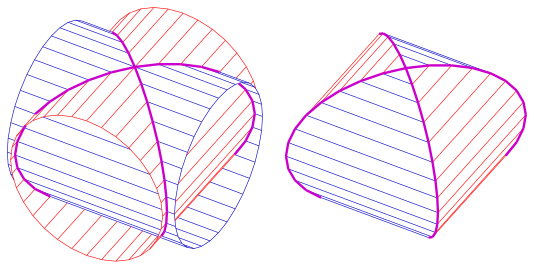
\includegraphics[width=0.5\paperwidth]{ex_3-10.png}
    \end{center}
    Note que a a região a ser integrada é formada por chapas quadradas de lado $2\sqrt{r^2-z^2}$.
    \begin{align*}
        V = \int_{-r}^r \int_{-\sqrt{r^2-z^2}}^{\sqrt{r^2-z^2}} \int_{-\sqrt{r^2-z^2}}^{\sqrt{r^2-z^2}} \diff x\,\diff y\,\diff z
            = \int_{-r}^r 4\,(r^2-z^2)\,\diff z
            = \frac{16}{3} r^3.
    \end{align*}
    
\end{solution}


% 3.11  % % % % % % % % % % % % % % % % % % % % %
% \setcounter{question}{7}
\question{
Calcule o volume do sólido delimitado inferiormente pelo cone $z = \sqrt{x^2 + y^2}$ e superiormente pela esfera $x^2 + y^2 + z^2 = 1$.
}

\begin{solution}
    Em coordenadas cilíndricas temos que o volume
    \begin{align*}
        V = \int_{0}^{\sqrt{2}/2}\int_{r}^{\sqrt{1-r^2}}\int_{0}^{2\pi} r\,\diff \theta\,\diff z\,\diff r
            = 2\pi \int_{0}^{\sqrt{2}/2} \left( r\sqrt{1-r^2} - r^2 \right) \diff r
            = \left(2-\sqrt{2}\right) \frac{\pi}{3}.
    \end{align*}
    Note que o limite de integração $0 \le r \le \sqrt{2}/2$ se deve ao fato que a esfera intersecta o cilindro em $r^2+r^2=1$, ou seja, em $r = \sqrt{2}/2$.
\end{solution}

% 3.12 % % % % % % % % % % % % % % % % % % % % %
% \setcounter{question}{5}
\question{
Calcule o volume do sólido delimitado superiormente pelo plano $z = 4$, inferiormente pelo parabolóide $z = 1 - x^2 - y^2$ e lateralmente pelo cilindro $x^2 + y^2 = 1$.
}

\begin{solution}
    Em coordenadas cilíndricas temos que o volume
    \begin{align*}
        V = \int_{0}^{1} \int_{1-r^2}^{4}\int_{0}^{2\pi} r\,\diff \theta\,\diff z\,\diff r
            = 2\pi \int_{0}^{1} \left( 3r+r^3 \right) \diff r
            = \frac{7\pi}{2}.
    \end{align*}
\end{solution}

\end{questions}


\setcounter{section}{2}
\section{Problemas}

\begin{questions}

% 3.1  % % % % % % % % % % % % % % % % % % % % %
% \setcounter{question}{0}
\question{
Determine a solução de quadrados mínimos do sistema sobredeterminado
\[
\left\{ \begin{array}{ccccc}
x_1 &+& x_2 & = & 1\\
x_1 &+& 2x_2 &=& 3 \\
x_1 &+& 3x_2 & = &6 \\
x_1 &+& 4x_2 &=& 10
\end{array} \right.
\]
Represente graficamente as retas que definem este sistema e a solução obtida. Interprete graficamente.
}
\begin{solution}
	Queremos resolver o problema
    $\displaystyle\min_{x\in\R^2}||Ax-b||_2^2$,
    onde
    \begin{align*}
        A = 
        \begin{bmatrix}
            1   & 1 \\
            1   & 2 \\
            1   & 3 \\
            1   & 4
        \end{bmatrix},
        \qquad
        b = 
        \begin{bmatrix}
            1\\ 3\\ 6\\ 10
        \end{bmatrix}.
    \end{align*}
    A solução é dada pela equação normal, ou seja, a solução $x^*$ deve satisfazer
    \[A^\top A x^* = A^\top b.\]
    Dessa forma,
    \begin{align*}
        \begin{bmatrix}
            4   &   10  \\
            10  &   30
        \end{bmatrix}
        x^* =
        \begin{bmatrix}
            20\\ 65
        \end{bmatrix}
        &\Rightarrow
        x^* = \frac{1}{120-100}
        \begin{bmatrix}
            30 & -10 \\
            -10 & 4
        \end{bmatrix}
        \begin{bmatrix}
            20 \\ 65
        \end{bmatrix}\\
        &\Rightarrow
        \boxed{
        x^* = 
        \begin{bmatrix}
            -5/2\\ 3
        \end{bmatrix}
        }.
    \end{align*}
    \begin{center}
    \begin{tikzpicture}
    \begin{axis}
    [
    grid = both,
    xmin = -7,  xmax = 0,
    ymin =  1, 	ymax = 5
    ]
        \addplot[domain=-9:0,samples=2]{1-x};
        \addplot[domain=-9:0,samples=2]{(3-x)/2};
        \addplot[domain=-9:0,samples=2]{(6-x)/3};
        \addplot[domain=-9:0,samples=2]{(10-x)/4};
        \addplot[draw=none,red,mark=*]coordinates{(-2.5,3)};
    \end{axis}
    \end{tikzpicture}
    \end{center}
    Podemos ver pelo gráfico que a solução aparenta ser o ponto no qual as retas se encontram próximas entre si e ainda está próximo das 6 soluções entre pares de equações.
\end{solution}

% 3.2 % % % % % % % % % % % % % % % % % % % % %
%\setcounter{question}{20}
\question{
Considere o problema de quadrados mínimos $\min \|Ax - b\|_2^2$ com
\[
A = \begin{bmatrix}
1 & 0 \\ 0 & 1 \\ 1 & 1
\end{bmatrix} \quad \text{e} \quad b = \begin{bmatrix}
1 \\ 1 \\ 0
\end{bmatrix}.
\]
Determine a solução ótima $x^\star$ deste problema. Verifique que $r^\star = b - Ax^\star$ é ortogonal às colunas de $A$. E se o vetor $b$ for trocado por $\hat b = [1~ 3~ 4]^\T$, o que acontece com a solução ótima e o resíduo associado? Interprete.
}
\begin{solution}
    Novamente, a solução é dada pela equação normal, ou seja, a solução $x^*$ deve satisfazer
    \[A^\top A x^* = A^\top b.\]
    Dessa forma,
    \begin{align*}
        \begin{bmatrix}
            2  &   1  \\
            1  &   2
        \end{bmatrix}
        x^* =
        \begin{bmatrix}
            1\\ 1
        \end{bmatrix}
        &\Rightarrow
        x^* = \frac{1}{4-1}
        \begin{bmatrix}
            2  & -1 \\
            -1 & 2
        \end{bmatrix}
        \begin{bmatrix}
            1 \\ 1
        \end{bmatrix}\\
        &\Rightarrow
        \boxed{
        x^* = 
        \begin{bmatrix}
            1/3\\ 1/3
        \end{bmatrix}
        }.
    \end{align*}
    Assim, $r^* = [2/3,2/3,-2/3]^\T$. Como $A^\T r^*= [0,0]^\T$, então $r^*$ é, de fato, ortogonal às colunas de $A$. Se $b$ for trocado por $\hat b$, então o sistema de equações passa a ter solução, ou seja, o resíduo associado será nulo.
\end{solution}

% 3.3  % % % % % % % % % % % % % % % % % % % % %
%\setcounter{question}{0}
\question{
Encontre a projeção de $b$ em ${\cal R}(A)$, sendo
\[
A = \begin{bmatrix*}[r]
1 & 1 \\ 2 & -1 \\ -2 & 4
\end{bmatrix*} \quad \text{e} \quad b = \begin{bmatrix}
1 \\ 2 \\ 7
\end{bmatrix}.
\]
Decomponha $b$ como $p+q$, com $p \in {\cal R}(A)$ e $q$ ortogonal à ${\cal R}(A)$. Em que subespaço está~$q$?
}
\begin{solution}
    A projeção de $b$ no conjunto $\cal{R}(A)$ pode ser encontrada através do seguinte problema de otimização
    $\displaystyle\min_{x\in\R^2}||Ax-b||_2^2$, de forma que a projeção é dada por $p=Ax^*$. Como visto anteriormente, a solução deve satisfazer a equação normal, ou seja, $A^\top A\,p = A^\top b.$ Assim,
   \begin{align*}
        \begin{bmatrix}
            9  &   -9  \\
            -9  &   18
        \end{bmatrix}
        x^* =
        \begin{bmatrix}
            -9\\ 27
        \end{bmatrix}
        &\Rightarrow
        x^* = \frac{1}{162-81}
        \begin{bmatrix}
            18  & 9 \\
            9   & 9
        \end{bmatrix}
        \begin{bmatrix}
            -9\\ 27
        \end{bmatrix}\\
        &\Rightarrow
        \boxed{
        x^* = 
        \begin{bmatrix}
            1\\ 2
        \end{bmatrix}
        }.
    \end{align*}
    Portanto, $p = Ax^* = [3,0,6]^\T$ e, por definição, $q = b-p = [-2,2,1]^\T$. Como $q$ é ortogonal às colunas de $A$, pois $A^\T q = [0,0]^\T$, então $q\in\cal{N}(A^\T)=\cal{R}(A)^\perp$.
\end{solution}

% 3.4 % % % % % % % % % % % % % % % % % % % % %
%\setcounter{question}{3}
\question{ \label{prob_reg_lin}
\textbf{Fórmulas de Regressão Linear} 
Considere o problema em que um conjunto de dados $(t^{(i)},y^{(i)})$, $i = 1,\cdots,N$, deve ser ajustado, no sentido de quadrados mínimos, por uma reta
\[
\phi(t) = x_1 + x_2 t.
\]
Construa o sistema normal associado a este problema e resolva-o para mostrar que os coeficientes ótimos são dados por
\[
x_1^\star = \frac{\left( \sum_{i = 1}^N \left(t^{(i)}\right)^2 \right) \left( \sum_{i =1}^N y^{(i)} \right) - \left( \sum_{i = 1}^N t^{(i)} \right) \left( \sum_{i =1}^N t^{(i)} y^{(i)} \right)}{N \sum_{i = 1}^N \left(t^{(i)}\right)^2 - \left( \sum_{i = 1}^N t^{(i)} \right)^2}
\]
e
\[
x_2^\star = \frac{N \left( \sum_{i =1}^N t^{(i)} y^{(i)} \right) - \left( \sum_{i = 1}^N t^{(i)} \right) \left( \sum_{i =1}^N y^{(i)} \right)}{N \sum_{i = 1}^N \left(t^{(i)}\right)^2 - \left( \sum_{i = 1}^N t^{(i)} \right)^2}.
\]
}

\begin{solution}
Para obter o melhor ajuste dos coeficientes $x_1,x_2$ devemos resolver o seguinte problema de otimização
\[
    \min_{x\in\R^2} \sum_{i=1}^N||\phi(t^{(i)})-y^{(i)}||_2^2
    ~\sim~ \min_{x\in\R^2} ||\Phi x - y||_2^2,
\]
onde
\[
    \Phi =
    \begin{bmatrix}
        1       & 1       & \cdots & 1 \\
        t^{(1)} & t^{(2)} & \cdots & t^{(N)}
    \end{bmatrix}^\T.
\]
  Logo, podemos usar a equação normal
  \begin{align*}
      x^* &= (\Phi^\T \Phi)^{-1}\Phi^\T y \\
        &=  \begin{bmatrix}
                N   & \sum_{i=1}^N t^{(i)} \\
                \sum_{i=1}^N t^{(i)} & \sum_{i=1}^N (t^{(i)})^2
            \end{bmatrix}^{-1}
            \begin{bmatrix}
                \sum_{i=1}^N y^{(i)}\\
                \sum_{i=1}^N t^{(i)}y^{(i)}\\
            \end{bmatrix}\\
        &=  \frac{1}{N\sum_{i=1}^N (t^{(i)})^2-\left(\sum_{i=1}^N t^{(i)}\right)}
            \begin{bmatrix}
                \sum_{i=1}^N (t^{(i)})^2 & -\sum_{i=1}^N t^{(i)} \\
                -\sum_{i=1}^N t^{(i)} & N
            \end{bmatrix}
            \begin{bmatrix}
                \sum_{i=1}^N y^{(i)}\\
                \sum_{i=1}^N t^{(i)}y^{(i)}\\
            \end{bmatrix}\\
        &=  \frac{1}{N\sum_{i=1}^N (t^{(i)})^2-\left(\sum_{i=1}^N t^{(i)}\right)}
            \begin{bmatrix}
                \left( \sum_{i = 1}^N \left(t^{(i)}\right)^2 \right) \left( \sum_{i =1}^N y^{(i)} \right) - \left( \sum_{i = 1}^N t^{(i)} \right) \left( \sum_{i =1}^N t^{(i)} y^{(i)} \right)\\
                N \left( \sum_{i =1}^N t^{(i)} y^{(i)} \right) - \left( \sum_{i = 1}^N t^{(i)} \right) \left( \sum_{i =1}^N y^{(i)} \right)
            \end{bmatrix}.
  \end{align*}
\end{solution}

% 3.10 % % % % % % % % % % % % % % % % % % % % %
\setcounter{question}{9}
\question{\textbf{Solução de Quadrados Mínimos de Norma Mínima.}
Quando a matriz $A \in \R^{m \times n}$ do problema de quadrados mínimos
\[
\min_{x \in \R^n} \|Ax - b\|_2^2,
\]
com $b \in \R^m$, não tiver posto completo, este problema não tem solução única. Neste caso, pode ser interessante encontrar o vetor $x^\star$ que é solução ótima deste problema e que tem norma Euclidiana mínima. Usando-se o sistema normal, podemos escrever este problema como
\[
\begin{array}{rl}
\min & \|x\|_2^2\\
\textrm{sujeito a} & A^\T A x = A^\T b.
\end{array}
\]
A restrição de igualdade deste problema pode ser removida parametrizando-se o núcleo de $A^\T A$; assim, obtemos um problema de otimização irrestrita. 

Encontre a solução de norma Euclidiana mínima para os problemas de quadrados mínimos definidos pelas matrizes abaixo:
\begin{parts}
\part $A = \begin{bmatrix} 1 & 1 & 0 \\ 1 & 1 & 0 \\
2 & 0 & 2 \end{bmatrix}$, $b = \begin{bmatrix*}[r]
1 \\ -1 \\ 1
\end{bmatrix*}$;
\part $A = \begin{bmatrix*}[r] 1 & 2 \\ 2 & 4 \\ -1 & -2 \end{bmatrix*}$, $b = \begin{bmatrix}
1 \\ 0 \\ 0
\end{bmatrix}$.
\end{parts}
}
\begin{solution}
	Para ambos itens, podemos resolver da seguinte maneira. Seja $F$ a matriz formada pelos vetores que geram $\cal{N}(A^\T A)$, então um problema de otimização equivalente pode ser enunciado como
	\[\min_{z\in\R^k} ||\bar x + Fz||_2^2
	~\sim~ \min_{z\in\R^k} ||Fz - (-\bar x)||_2^2,\]
	onde $k$ é $n$ menos o posto da matriz $A^T A$ e $\bar x$ é uma solução particular do sistema de equações normais. Note que podemos colocar esse problema equivalente como um problema de quadrados mínimos e resolvê-lo usando a equação normal, ou seja, \[F^\T F z^* = F^\T (-\bar x).\]
	\begin{parts}
	    \part Montando o sistema de equações normais $A^\T A x = A^\T b$, temos que
	    \begin{align*}
	        \begin{bmatrix}
	            6 & 2 & 4 \\
	            2 & 2 & 0 \\
	            4 & 0 & 4
	        \end{bmatrix} x
	        =
	        \begin{bmatrix}
	            2\\ 0\\ 2
	        \end{bmatrix}
	    \end{align*}
	    Nesse problema, $k=1$, logo, seja $x_1=z$, então da segunda linha de equações, temos que $x_2=-z$ e da terceira linha $x_3 = 1/2-z$.
	    Logo,
	    \[
	        x = 
	        \begin{bmatrix}
	            z\\ -z\\ 1/2-z
	        \end{bmatrix}
	        =
	        \underbrace{\begin{bmatrix}
	            0\\ 0\\ 1/2
	        \end{bmatrix}}_{\bar x}
	        +
	        \underbrace{\begin{bmatrix}
	            1\\ -1\\ -1
	        \end{bmatrix}}_{F} z.
	    \]
	    Assim,
	    $
	        z^* = (F^\T F)^{-1} F^\T (-\bar x)
	            = (1/3) (1/2)
	            = 1/6.
	    $\\
	    Portanto, $\boxed{x^* = [-1/6, 1/6, 1/3]^\T}$.
	    
	    \part  Montando o sistema de equações normais $A^\T A x = A^\T b$, temos que
	    \begin{align*}
	        \begin{bmatrix}
	            6  & 12 \\
	            12 & 24
	        \end{bmatrix} x
	        =
	        \begin{bmatrix}
	            1\\ 2
	        \end{bmatrix}
	    \end{align*}
	    Nesse problema, $k=1$, logo, seja $x_2=z$, então da primeira linha de equações, temos que $x_1=1/6-2z$.
	    Logo,
	    \[
	        x = 
	        \begin{bmatrix}
	            1/6-2z\\ z
	        \end{bmatrix}
	        =
	        \underbrace{\begin{bmatrix}
	            1/6\\ 0
	        \end{bmatrix}}_{\bar x}
	        +
	        \underbrace{\begin{bmatrix}
	            -2\\ 1
	        \end{bmatrix}}_{F} z.
	    \]
	    Assim,
	    $
	        z^* = (F^\T F)^{-1} F^\T (-\bar x)
	            = (1/5) (1/3)
	            = 1/15.
	    $\\
	    Portanto, $\boxed{x^* = [1/30, 1/15]^\T}$.
	\end{parts}
\end{solution}

% 3.11 % % % % % % % % % % % % % % % % % % % % %
%\setcounter{question}{74}
\question{\textbf{Sistemas Subdeterminados: Solução de Norma Mínima e Problemas de Quadrados Mínimos com Regularização de Tikhonov.}
O problema discutido acima está relacionado com o seguinte problema: dado um sistema linear $Ax = b$, com $A \in \R^{m \times n}$ e $b \in \R^m$ e $m < n$. Se este sistema for compatível, então ele admite infinitas soluções; vamos assumir que o posto de $A$ é completo, o que assegura essa propriedade. Dentre todas estas soluções, desejamos determinar a que possui a menor norma, ou seja, desejamos resolver o problema
\[
\begin{array}{rl}
\min & \|x\|_2^2\\
\textrm{sujeito a} & Ax = b.
\end{array}
\]
\begin{parts}
\part Interprete este problema geometricamente.
\part Mostre que a solução ótima deste problema é dada por $x^\star = A^\T (AA^\T)^{-1}b$; para tanto, tome outra solução arbitrária deste sistema $x = x^\star + z$, com $z$ tal que $Az = 0$ e mostre que a norma é maior que ou igual à norma de $x^\star$.

\part Este problema tem uma relação interessante com o problema de quadrados mínimos com {\em regularização de Tikhonov}:
\[
\min \|Ax - b\|_2^2 + \lambda \|x\|_2^2,
\]
em que $\lambda > 0$ é um parâmetro definido pelo projetista. A regularização de Tikhonov evita que os coeficientes de ajuste do problema de quadrados mínimos sejam arbitrariamente grandes, impondo um certo {\em trade-off} entre a norma do resíduo e a norma da solução.

Use as condições de otimalidade para determinar a solução ótima deste problema. O que acontece com esta solução se $\lambda \to 0$?
\end{parts}
}
\begin{solution}
\begin{parts}
	\part Esse problema é equivalente à encontrar o ponto do conjunto $\{x\in\R^n\mid Ax=b\}$ que esteja mais próximo à origem, ou seja, é a projeção da origem nesse conjunto.
	
	\part
	\begin{proof}
	Primeiramente mostramos que, de fato, $Ax^*=b$.
	    \[Ax^* = AA^\T (AA^\T)^{-1}b = b,\]
	pois $AA^\T$ é inversível, dado que $A$ tem posto completo.
	Agora mostremos que $||x^*||_2\le||x||_2$ para todo $x$ que satisfaaça $Ax=b$. Seja $z\in\mathscr{N}(A)$,
		\begin{align*}
	    ||x||_2^2 &= ||x^*+z||_2^2\\
	        &= (x^*+z)^\T(x^*+z)\\
	        &= ({x^*})^\T x^*+2(x^*)^\T z+z^\T z\\
	        &= ||x^*||_2^2 + 2(A^\T (AA^\T)^{-1}b)^\T z + ||z||_2^2\\
	        &= ||x^*||_2^2 + 2((AA^\T)^{-1}b)^\T \underbrace{Az}_0 + ||z||_2^2\\[-4mm]
	        &= ||x^*||_2^2+||z||_2^2\\
	        &\ge ||x^*||_2^2.
	\end{align*}
	\end{proof}

	\part A função objetivo pode ser re-escrita como
	\begin{align*}
	    f_0(x) &= (Ax-b)^\T(Ax-b)+\lambda x^\T x\\
	        &= x^\T A^\T A x - 2 x^\T A^\T b + b^\T b + \lambda x^\T x\\
	        &= x^\T (A^\T A + \lambda I_n) x - 2 x^\T A^\T b + b^\T b,
	\end{align*}
	onde $I_n$ é a matriz identidade. Portanto, o gradiente é dado por
	\[ \nabla f_0(x) = 2(A^\T A + \lambda I_n)x-2A^\T b.\]
	Resolvendo $\nabla f_0(x^*) = 0$, obtemos
	\[x^* = (A^\T A+\lambda I_n)^{-1} A^\T b.\]
	Note que a matriz $(A^\T A+\lambda I_n)$ é inversível e definida positiva, dado que $\det(A^\T A)=0$ e $\lambda>0$. Esse problema é convexo, então não é necessário checar as condições de segunda ordem.
	
	Como esperado, se $\lambda\to 0$, $x^*$ converge para a solução do item anterior. O motivo é que estamos dando um peso grande para o termo $||Ax-b||_2^2$ ao dar um peso pequeno para $||x||_2^2$, ou seja, o problema se torna equivalente à minimizar $||x||_2^2$ restrito à $Ax=b$. É importante notar que $\lambda$ não pode ser igual à zero, pois ao contrário de $AA^\T$, a matriz $A^\T A$ \textbf{não} é inversível.
\end{parts}
\end{solution}

% 3.14 % % % % % % % % % % % % % % % % % % % % %
\setcounter{question}{13}
\question{
Considere o problema de quadrados mínimos $\|b - Ax\|_2^2$ com $A$ e $b$ dados por
\[
A = \begin{bmatrix}
1 & 1 \\ 0 & 0 \\ 1 & 1 + \alpha
\end{bmatrix}, \quad b = \begin{bmatrix}
2 \\ 1 \\ 0
\end{bmatrix}.
\]
\begin{parts}
\part Para que valores de $\alpha \in \R$ este problema possui solução única?
\part Assumindo que $\alpha \neq 0$, resolva o problema de quadrados mínimos dado acima e calcule o resíduo ótimo. O resíduo depende de $\alpha$?
\part Investigue o que acontece com a solução $x^\star$ encontrada acima quando $\alpha \to 0$. O que acontece com o resíduo ótimo?
\end{parts}
}
\begin{solution}
\begin{parts}
    \part Usando a equação normal $A^\T A x^* = A^T b$, temos que
    \[
    \begin{bmatrix}
        2           & 2+\alpha      \\
        2+\alpha    & 1+(1+\alpha)^2
    \end{bmatrix} x^*
    =
    \begin{bmatrix}
    2\\ 2
    \end{bmatrix}.
    \]
    Esse problema tem solução única se, e somente se, $\det(A^\T A) \neq 0$. Como $\det(A^\T A) = \alpha^2$, então o problema tem solução única para todo $\alpha\neq 0$.
    
    \part Resolvendo a equação normal, temos que
    \begin{align*}
        x^* &= (A^\T A)^{-1}A^\T b\\
            &= \frac{1}{\alpha^2}
                \begin{bmatrix}
                    2+2\alpha+\alpha^2 & -(2+\alpha)\\
                    -(2+\alpha) & 2
                \end{bmatrix}
                \begin{bmatrix}
                    2\\ 2
                \end{bmatrix}\\
            &= \frac{2}{\alpha}
            \begin{bmatrix}
                1+\alpha\\ -1
            \end{bmatrix}.
    \end{align*}
    O resíduo ótimo é dado por
    \begin{align*}
        r^* = b-Ax^* = 
        \begin{bmatrix}
           2\\ 1\\ 0
        \end{bmatrix}
        - \dfrac{2}{\alpha}
        \begin{bmatrix}
            \alpha\\ 0\\ 0
        \end{bmatrix}
        =
        \begin{bmatrix}
            0\\ 1\\ 0
        \end{bmatrix}.
    \end{align*}
    Assim, o resíduo $||r^*(\alpha)||_2=1$ coincidentemente não depende de $\alpha$.
    
    \part Esse limite não existe, pois $\lim_{\alpha\to 0}1/\alpha$ é indeterminado. Quando $\alpha=0$ a solução tem 1 grau de liberdade, já que a solução da equação normal não é única para esse caso, então era de se esperar que o limite não deveria existir.
    
    Em relação ao resíduo, o limite existe $\lim_{\alpha\to 0}||r^*(\alpha)||_2=1$. Porém, ele é diferente do resíduo quando resolvemos o problema para $\alpha = 0$, em que encontraríamos $||r^*(0)||_2=2$. Dessa forma, $\lim_{\alpha\to 0}||r^*(\alpha)||_2 \neq ||r^*(0)||_2$.
\end{parts}

\end{solution}

\end{questions}


% \setcounter{section}{4}
% \section{Exercícios Teóricos}
% \begin{questions}

% 5.27 % % % % % % % % % % % % % % % % % % % % %
\setcounter{question}{26}
\question{
Se $X$ é uniformemente distribuída em $(a, b)$, qual variável aleatória que varia linearmente com $X$ é uniformemente distribuída em $(0, 1)$?
}
\begin{solution}
Seja $Y = (X-a)/(b-a)$, então
\begin{align*}
	F_Y(y) &= P(Y\le y) = P((X-a)/(b-a) \le y)\\
    	&= P(X \le (b-a)\,y+a) = F_X((b-a)\,y+a).
\end{align*}
Derivando os dois lados da equação em relação à $y$ obtemos que
\begin{align*}
	f_Y(y) =  (b-a)f_X((b-a)\,y+a) =
    \begin{cases}
    	1, &\text{se }y\in(0,1);\\
        0, &\text{caso contrário.}
    \end{cases}
\end{align*}
Logo, $Y$ é uniformemente distribuída em $(0,1)$.\\[1mm]
\textit{Observação:} outra opção é fazer $Y = (b-X)/(b-a)$.
\end{solution}

% 5.29 % % % % % % % % % % % % % % % % % % % % %
\setcounter{question}{28}
\question{
Seja $X$ uma variável aleatória contínua
com função distribuição cumulativa $F$.
Defina a variável aleatória $Y$ como $Y = F(X)$.
Mostre que $Y$ é uniformemente distribuída em $(0, 1)$.
}
\begin{solution}
	Por simplicidade, vamos supor que $F: \mathbb{R} \to [0,1]$ seja estritamente crescente. Logo, $F$ é inversível e para $y \in (0,1)$,
	\begin{align*}
		F_Y(y) = P(Y\le y) = P(F(X)\le y) = P(X \le F^{-1}(y)) = F(F^{-1}(y)) = y.
	\end{align*}
    Dessa forma, quando $y \in \mathbb{R}$,
    \begin{align*}
    	F_Y(y) =
        \begin{cases}
    	0, &\text{se }y \le 0;\\
        y, &\text{se }0 < y < 1;\\
        1, &\text{se }y \ge 1;\\
    	\end{cases}
    \end{align*}
    o que caracteriza uma distribuição uniforme em $(0,1)$.\\[1mm]
    \textit{Observação:} Isso também acontece quando $F$ não é inversível.
\end{solution}

% 5.30 % % % % % % % % % % % % % % % % % % % % %
%\setcounter{question}{28}
\question{
Suponha que $X$ tenha função densidade
de probabilidade $f_X$. Determine a função
densidade de probabilidade da variável
aleatória $Y$ definida como $Y = aX + b$.
}
\begin{solution}
	Seja $a>0$,
	\begin{align*}
		F_Y(y) = P(Y\le y) = P(aX+b\le y) = P(X\le (y-b)/a) = F_X((y-b)/a).
	\end{align*}
    Derivando ambos lados da equação em relação à $y$ leva à
    \begin{align*}
    	f_Y(y) = \frac{f_X((y-b)/a)}{a}.
    \end{align*}
    Por outro lado, se $a<0$, então
    \begin{align*}
    	F_Y(y) &= P(X\ge (y-b)/a) = 1-P(X<(y-b)/a) = 1-F_X([(y-b)/a]^-)\\
        	&= 1-F_X((y-b)/a) \quad\text{(a variável aleatória é contínua).}
    \end{align*}
    Novamente, derivando ambos lados da equação em relação à $y$ leva à
    \begin{align*}
    	f_Y(y) = \frac{f_X((y-b)/a)}{-a}.
    \end{align*}
    Portanto, quando $a\neq 0$,
    \begin{align*}
    	f_Y(y) = \frac{f_X((y-b)/a)}{|a|}.
    \end{align*}
\end{solution}

\end{questions}
%\newpage

\end{document}